% Preamble
\documentclass[../Relazione_circuiti]{subfiles}

% Packages

\graphicspath{{\subfix{../images/}}}

% Document
\begin{document}

\subsection{Analisi preliminare qualitativa}

  \begin{figure}[H]
    \centering

    \begin{subfigure}[b]{0.3\textwidth}
      \centering
      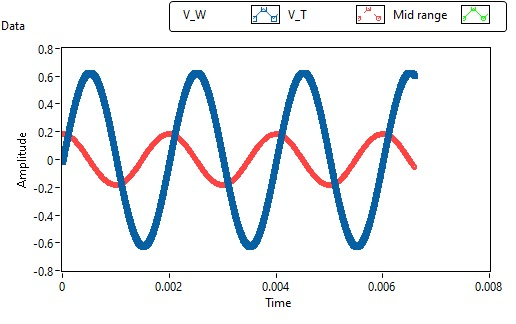
\includegraphics[width=\textwidth]{Cross_waveform_500.jpeg}

      \caption{Segnali a 500Hz}
      \label{fig:signal_500}

    \end{subfigure}
    \hfill
    \begin{subfigure}[b]{0.3\textwidth}
      \centering
      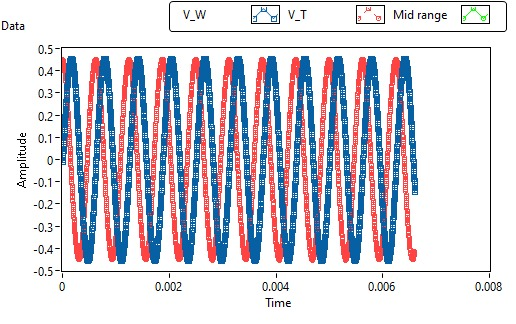
\includegraphics[width=\textwidth]{Cross_waveform_1600.jpeg}

      \caption{Segnali a 1600Hz}
      \label{fig:signal_1600}

    \end{subfigure}
    \hfill
    \begin{subfigure}[b]{0.3\textwidth}
      \centering
      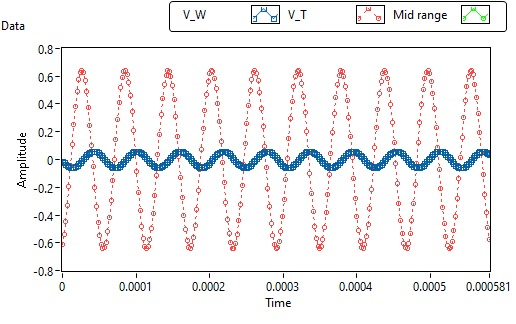
\includegraphics[width=\textwidth]{Cross_waveform_17000.jpeg}

      \caption{Segnali a 17kHz}
      \label{fig:signal_17k}

    \end{subfigure}
    \hfill

    \caption{Segnali osservati sui rami Woofer (blu) e Tweeter (rosso)
      a frequenza fissata. Le incertezze non sono visibili a causa della scala.}

    \label{fig:signal_waveforms}

  \end{figure}


  La Fig. \ref{fig:signal_waveforms} mostra la forma d'onda dei segnali osservati sui rami Woofer e Tweeter in risposta
  ad un segnale sinusoidale.
  La Fig. \ref{fig:signal_1600} mostra il comportamento nei pressi della frequenza di cross attesa, la Fig.
  \ref{fig:signal_500} a 1/3 e la Fig. \ref{fig:signal_17k} a circa 10 volte.

  Si osserva (Fig. \ref{fig:signal_1600}) che, coerentemente con quanto atteso, i segnali hanno ampiezza simile nei
  pressi di $f_{cross}$.
  A basse frequenze si osserva (Fig. \ref{fig:signal_500}) un'attenuazione del 60\% dell'ampiezza sul ramo Tweeter e
  nessuna alterazione sul Woofer, ad alte frequenze un'attenuazione sul Woofer dell'86\% e nessuna sul Tweeter (Fig.
  \ref{fig:signal_17k}). Questa prima analisi qualitativa è in accordo con la teoria.

\subsection{Analisi della frequenza misurata}

\subsection{Analisi dell'ampiezza}

  \begin{figure}[H]
    \centering

    \begin{subfigure}[t]{=0.49\textwidth}

      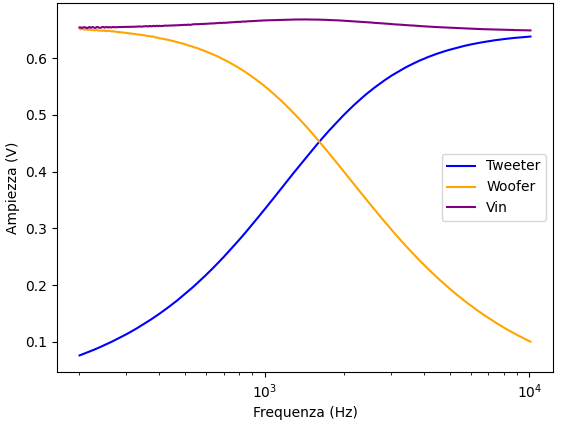
\includegraphics[width=\textwidth]{cross_dataonly.png}

      \caption{Andamenti sperimentali di Tweeter, Woofer e Vin (segnale in ingresso nel filtro,
        a valle della resistenza interna del generatore).}
      \label{fig: amplitude_dataonly}

    \end{subfigure}
    \hfill
    \begin{subfigure}[t]{=0.49\textwidth}

      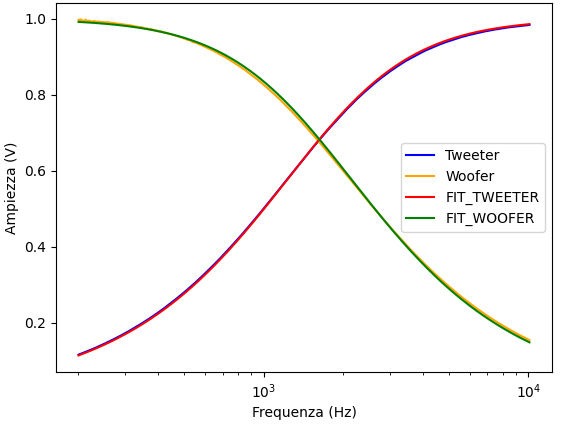
\includegraphics[width=\textwidth]{cross_gain_amplitude.png}

      \caption
      {Andamenti sperimentali e fit dei guadagni in tensione.}
      \label{fig:cross_gain}
    \end{subfigure}

    \caption{Ampiezza misurata in funzione della frequenza (asse della frequenza in scala logaritmica). A causa della scala le incertezze sulle singole misure non sono visibili. L'andamento è rappresentato da una
      linea continua a causa dell'alta densità di punti.}
    \label{fig:cross_amplitude}

  \end{figure}

  La Fig. \ref{fig:cross_amplitude} mostra l'andamento di ampiezza dei segnali filtrati in funzione della frequenza.

  La relazione funzionale Ampiezza massima-Frequenza (misurata ai capi della resistenza di carico dei rami) dipende
  dalla tensione in ingresso sul filtro $V_{in}$.
  Tuttavia, a causa della presenza della resistenza interna nel generatore e come visibile in Fig.
  \ref{fig: amplitude_dataonly}, la $V_{in}$
  dipende dalla frequenza ed assumerla costante potrebbe introdurre errori.
  Pertanto abbiamo determinato i guadagni in tensione (Fig. \ref{fig:cross_gain}
  ) dividendo le ampiezze osservate per il valore di $V_{in}$
  osservato alla relativa frequenza, propagando le incertezze in quadratura. Gli andamenti seguiti da queste funzioni sono: 

  \begin{equation}
    \label{eq:gain_woofer}
    G_{woofer} = \frac{1}{\sqrt{R^2+(\omega L)^2}}
  \end{equation}

  \begin{equation}
    \label{eq:gain_tweeter}
    G_{tweeter} = \frac{1}{\sqrt{R^2+(\frac{1}{\omega C})^2}}
  \end{equation}

%dove $V_{in}$ rappresenta la tensione in ingresso. %(assunta costante) pari a 0.65, osservata nel ramo Woofer nel
%    limite di basse frequenze e nel ramo Tweeter nel limite di alte frequenze.

%Le funzioni guadagno si ottengono semplicemente dividendo le eq date per vin (NOTA: da riscrivere, non voglio
%    duplicare le equazioni)

  È stato effettuato un fit ai parametri $L$ e $C$ ($R$ fissata).
  Da essi è stata poi ricavata la frequenza di crossover secondo l'Eq. \eqref{eq:f_cross}.

  \begin{table}[H]
    \centering

    \begin{tabular}{c | c }

      %Heading
      Grandezza & Valore                 \\

      L         & $(10.13 \pm 0.01)$ mH  \\
      C         & $(953.39 \pm 0.05)$ nF \\
      $f_{cross}$ & $(1619 \pm 2)$ Hz \\
	$\chi^2_{woofer}$	& 15755.73  \\
	$\chi^2_{tweeter}$ & 19483.52  

    \end{tabular}

    \caption{Risultati del fit alle funzioni guadagno in tensione}
    \label{tab:fit_amplitude}

  \end{table}

  La Tab. \ref{tab:fit_amplitude} mostra i risultati del fit.
  Si osserva che la frequenza ottenuta non risulta compatibile con il valore teorico stimato \theoryF.
  Tuttavia, l'andamento della curva $V_{in}$ ci fornisce un metodo ulteriore per determinare la frequenza di cross.
  Infatti, si dimostra che a tale frequenza l'impedenza totale del filtro è massima.
  Usando la legge di Ohm simbolica, ne segue che la tensione ai capi del filtro deve essere massima.
  Cercando il massimo della curva sperimentale, otteniamo il valore $(1434 \pm 8) \;$ Hz.
  L'incertezza è stata determinata considerando metà del passo di scansione utilizzato nei pressi di quella frequenza
  (come descritto in sezione 2, non è costante). Risulta pertanto essere un'incertezza massima.
  


\subsection{Analisi della fase}

  \begin{figure}[H]
    \centering

    \begin{subfigure}{=0.49\textwidth}
      \centering
      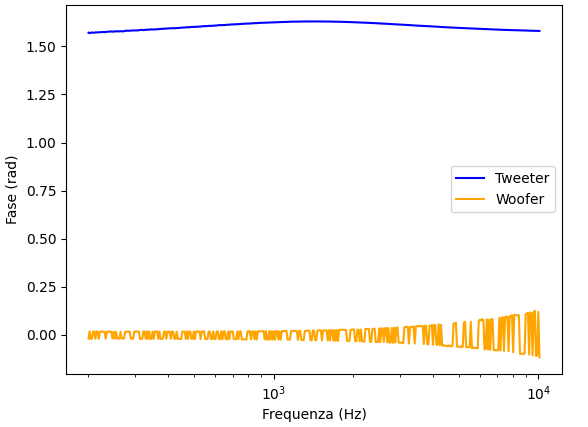
\includegraphics[width=.99\textwidth]{phase_dataonly.png}
      \caption{Sfasamento Tweeter-Woofer (solo dati)}
      \label{fig: pdiff_dataonly}

    \end{subfigure}
    \hfill
    \begin{subfigure}{=0.49\textwidth}
      \centering
      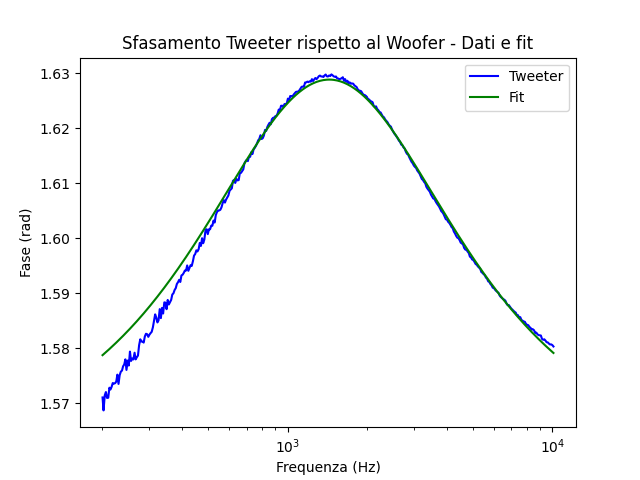
\includegraphics[width=.99\textwidth]{phase_cross.png}
      \caption{Dati e sovrapposizione con fit}
      \label{fig: pdiff_fit_data}

    \end{subfigure}

    \caption{Fase del Tweeter misurata rispetto al Woofer (blu). Fase del Woofer misurata rispetto se stesso (giallo)
      . La frequenza è in scala logaritmica. Le incertezze non sono visibili a causa della scala.}
    \label{fig: phase_diff}

  \end{figure}

  La Fig.\,\ref{fig: pdiff_dataonly} mostra lo sfasamento relativo Tweeter-Woofer (curva Tweeter in figura), che segue la
  relazione definita dall'Eq.\,\eqref{eq:p_diff}.
  La Fig.\,\ref{fig: pdiff_dataonly} mostra lo sfasamento relativo Tweeter-Woofer (curva Tweeter in figura).
  Ai dati è stata assegnata un'incertezza casuale stimata mediante fit alla forma d'onda osservata per ogni frequenza,
  come descritto in sezione 2.  
  
Inoltre, poiché l'acquisizione dei due canali non è simultanea ma sequenziale (mediante multiplexer che itera sui
  canali Analog Input) si ha che tra due canali acquisiti consecutivamente (come nel nostro caso) vi è uno sfasamento
  temporale tra l'inizio delle due acquisizioni, che risulta essere pari a $\tau_{aq}=1 \mu \mathrm{S}$
      secondo le specifiche di ELVIS, che si riflette in un errore sistematico sulla fase, che risulta essere inferiore
      al valore vero.

      Questo è stato corretto aggiungendo alla fase misurata  $ 2 \pi f \tau_{aq}$, dove $f$
      rappresenta la frequenza del segnale (si veda l'appendice per una spiegazione approfondita).

      In Fig.\,\ref{fig: phase_diff}
      si nota che la fase del Woofer rispetto se stesso, che ci aspettavamo essere 0 poiché il trigger è sul medesimo
      canale, risulta in realtà non nulla ma oscillante attorno a questo valore. L'ampiezza di dette oscillazioni
      aumenta all'aumentare della frequenza. Questo fenomeno è stato osservato anche sulla fase del tweeter e la cosa è
      coerente con il fatto che la fase del tweeter è misurata relativamente al Woofer: una fluttuazione nello 0 della
      fase si ripercuote su tutte le altre misure. Abbiamo corretto queste fluttuazioni sul canale Tweeter sottraendo i
      valori misurati sul canale Woofer. Questo non ha influenzato il valore medio di sfasamento del Tweeter ad una data
      frequenza poiché la fase del Woofer è in media 0.  
  
  
  Effettuando un fit con l'Eq.\,\eqref{eq:p_diff}, fissando $R$
      poiché la frequenza di cross non dipende da esso, abbiamo
      ricavato i valori $L$ e $C$, e grazie all'Eq.\,\eqref{eq:p_diff_cross} abbiamo stimato la frequenza di cross.



  \begin{table}[H]
    \centering

\begin{tabular}{c | c }
%Heading
Grandezza & Valore  \\
\hline
L & $ 11.82 \pm 0.03 $  mH \\
C & $ 1.037 \pm 0.002 $  $\mathrm{\mu}$F \\
$f_{cross}$ & $ 1437 \pm 2$  Hz \\
$\widetilde{\chi}^2$ & $49.62$ 

    \end{tabular}
    \caption{Risultati del fit dell'Eq.\,\eqref{eq:p_diff}}
    \label{tab:fit_phase}

  \end{table}
%ribadisco per chiarezza


%discussione fit
Il valore ottenuto è risultato compatibile con il valore teorico atteso \theoryF. La stima mediante analisi della fase risulta tuttavia più precisa, dato che presenta un'incertezza percentuale dello 0.14\% contro lo 0.69\% del valore teorico. Il $\chi^2$ ottenuto risulta molto maggiore del valore ottimale pari a 1.
 In effetti, il fit si discosta in maniera significativa dai dati a basse frequenze, risultando tuttavia più accurato nei pressi della frequenza di cross e ad alte frequenze. Tuttavia questo non inficia la compatibilità del valore ottenuto con il valore atteso per la frequenza di crossover.
 Possiamo pertanto ritenere che il modello descriva adeguatamente il comportamento reale nei pressi della frequenza di cross e a frequenze superiori ad essa.


\end{document}